\documentclass[11pt]{article}
\usepackage[
    top = 1in,
    bottom = 1.25in,
    left = 1.25in,
    right = 1.25in
]{geometry}
\usepackage[]{amsmath, amssymb}
\usepackage[]{graphicx}
    \graphicspath{{./figures/}}
\usepackage[]{subcaption}
\usepackage[]{float}
\usepackage[]{siunitx}
\usepackage[style=authoryear,maxbibnames=99,backend=biber]{biblatex}
\addbibresource{references.bib} % replace by the name of your .bib file
\usepackage[]{lipsum}
\usepackage[]{array}
    \renewcommand{\arraystretch}{1.2}
    \usepackage[table,dvipsnames]{xcolor}
    \definecolor{sky}{RGB}{87, 191, 255}
\usepackage[
    colorlinks = true,
    linkcolor = MidnightBlue,
    urlcolor = MidnightBlue,
    citecolor = MidnightBlue
]{hyperref}

% \setlength{\parindent}{0pt}
\setlength{\parskip}{0.5em}
\newcommand{\size}{\Large}

\title{Radio Astronomy Imaging with LOFAR \\ Statistical Digital Signal Processing - EE4795}
\author{Alfonso Sánchez Rodríguez}

\begin{document}

\maketitle
\cleardoublepage
\setcounter{page}{1}

\section{Introduction}
\label{s:introduction}

The LOw-Frequency ARray (LOFAR) is an European radio interferometer designed to observe the universe in the 10-240 MHz range~\parencite{van_haarlem_lofar_2013}.
The network includes both Low Band Antennas (LBAs), designed to operate in the 10-90 MHz range, and High Band Antennas (HBAs), optimized for the 110-250 MHz range.
LOFAR antennas are organized into small clusters known as stations.
The geographical distribution of the stations is such that they approximately form a logarithmic spiral centered in a 320 m diameter region known as the SuperTerp.
This project investigates different approaches to produce a radio-astronomical image based on measurements from 273 LBAs located within the SuperTerp.

In the context of this project, a radio-astronomical image is a graphical representation of the observed brightness of the sky at a given frequency and epoch~\parencite{bhattacharyya_signal_2013}.
Each pixel in the image corresponds to a particular direction of observation, and its color encodes the intensity of the received radiation when measuring along it.
Since the idea of radio-interferometry is to combine measurements from multiple antennas to make them behave as a single detector, translating the raw detections of individual LBAs into an image requires some processing steps.
One of such steps is \emph{correlation}: the process of computing the cross-correlation between simultaneous\footnote{When calibrated for geometric delays} recordings from different antennas~\parencite{thompson_interferometry_2017}.
The cross-correlations that result from this process are known as complex visibilities, and linked to the measured intensity through an inverse Fourier transform.
Our input in this project is a matrix of complex visibilities derived from measurements performed with the 273 LBAs mentioned above, at a single epoch and frequency.

The fact that interferometric networks are made up of a finite set of antennas with a particular geographical distribution implies that the correlation of their measurements yields a filtered version of the complex visibility.
More concretely, and following the terminology in~\textcite{thompson_interferometry_2017}, the output of the correlator is the product of the complex visibility and the (weighted) \emph{transfer function} of the array.
The inverse Fourier transform of the measured visibility thus yields the actual intensity distribution convolved with the Fourier transform of the (weighted) transfer function or \emph{dirty beam}.
The process of recovering the actual intensity field from the \emph{dirty image} (i.e. intensity convolved with dirty beam) falls out of the scope of this project.

With this context in mind, this project aims to investigate different approaches to produce a dirty image from a matrix of complex visibilities derived from one epoch of LOFAR observations.
Section~\ref{s:methods} introduces the different imaging algorithms and the three metrics we defined to assess their performance.
The resulting images, their metrics and their interpretation are covered in section~\ref{s:results}.

% This project investigates different approaches to produce a radio-astronomical image from LOFAR observations.
% Starting from a matrix of complex visibilities, we use three different algorithms to produce a dirty image.
% The performance of the algorithms is discussed in terms of quantitative metrics and a visual comparison of the images.

% \textcolor{red}{\textbf{What problem am I trying to solve?}}


% \textcolor{red}{What type of comparison am I supposed to perform? Do I need to discuss the different types of arctifacts you get, the different problems to which the methods are susceptible, the quality of the image\ldots This is not something I can decide myself. It is a requirement.}

% The goal of this project is investigating different approaches to produce an image from a set of LOFAR measurements using power spectrum estimation techniques. We will start with an overview of the high-level process that is common to all the approaches, comment how each of the approaches introduces particularities in this high-level process, produce the image with all of them and then discuss the variability in the output and implications. The general goal is getting a better understanding of the output's sensitivity to the processing approach.

% \subsection{General information about LOFAR}

% The SuperTerp is the name of the circle that always appears in the pictures, it includes the shortest baselines in the array and can be combined to effectively for a single, large station --discussed in subsection 12.10 of~\textcite{van_haarlem_lofar_2013}.

% LOFAR antenna stations perform the same basic functions as the dishes of a conventional interferometric radio telescope. Like traditional radio dishes, these stations provide collecting area and raw sensitivity as well as pointing and tracking capabilities. However,the antennas within a LOFAR station do not physically move. Instead, pointing and tracking are achieved by combining signals from the individual antenna elements to form a \textcolor{red}{\textbf{phased array}} using a combination of analog and digital beamforming techniques (see Thompson et al. 2007).

% LOFAR stations are classified as core, remote or international according to their distance to the center of the array.
% All LOFAR stations in the Netherlands have 96 Low Band Antennas (LBA), 48 High Band Antennas (HBA) and 48 digital Receiver Units (RCU).
% Operationally, the LBA dipoles are grouped into an inner circle and an outer annulus each consisting of 48 dipoles and identified as the “LBA Inner” and “LBA Outer” configurations, respectively. These two configurations result in different FoVs, and potentially sensitivity (due to mutual coupling of closely spaced antennas), and can be selected by the observer during the observation specification process.
% The set of measurements we use in this project were obtained with the subset of LBA core antennas in the SuperTerp, operating in outer configuration.

% The operational range of the LBAs is of 30-80 MHz, and the peak of their response curve is at 58 MHz. This is very close to the value of \texttt{central\_channel\_frequency} in the data file that we are using as input, of $\sim 58.97~\unit{MHz}$.

% The LBA dipoles in a given LOFAR station can easily be correlated to provide all-sky maps on timescales of seconds (see Fig. 6). (\textcolor{red}{\textbf{probably related to our application}})

% \subsection{Information about DSP in LOFAR}

% The raw detections are filtered, amplified, converted to base-band frequencies and then digitized at the RCUs (details in 4.4 of~\textcite{van_haarlem_lofar_2013}). (\textcolor{red}{\textbf{The discussion became very technical and I don't think it makes sense for me to go that deep into it}})

% In classical radio telescopes an XF correlator was generally used, meaning that first the correlation and integration of the signals was done in the time domain (X) and afterwards the Fourier transform (F) was accomplished to get a cross power spectrum out of the correlator (Romney 1999). This option is still an economically attractive technique for radio telescopes with a limited number of antennas (input signals to the correlator). However, for LOFAR an FX correlator (first Fourier transform and then correlating the resulting channels) is favorable in terms of processing at the expense of data transport (the signals must be regrouped per channel instead of per antenna, resulting in a transpose operation). Using only a Fourier transform in the FX correlator leads to a significant amount of leakage between the channels. Therefore it was chosen to use filter banks before the correlator. This architecture is also known as an HFX (Hybrid FX correlator) architecture (Romney 1999).

% The correlator calculates the auto and cross correlations between all pairs of stations, for each channel and for each polarization (XX, XY, YX, and YY). A correlation is the complex product of a sample from one station and the complex conjugate of a sample from the other station. \ldots Since the correlation of station S1 and S2 is the conjugate of the correlation of station S2 and S1, we only compute the correlations for S1 ≤ S2.

% \subsection{Observing modes}

% \textcolor{red}{\textbf{Stopped reading at the start of this section}}

% \section{Motivation}

% \textcolor{red}{\textbf{Should I do some literature review about the different approaches to understand the motivation for having developed them and report that? Otherwise not clear what to do}}

% Why is this an important problem to solve?

\section{Methodology}
\label{s:methods}

The following section covers the formulation of the three algorithms we used to produce dirty images, and the description of the metrics we defined for their assessment and the way in which we computed them.
The implementation of these algorithms can be found, together with the scripts used to generate the images, in \href{https://github.com/alfonsoSR/sdsp-assignment}{https://github.com/alfonsoSR/sdsp-assignment}.

\subsection{Imaging algorithms}
\label{ss:methods:algorithms}

As we discussed in section~\ref{s:introduction}, the measured intensity along a certain direction, $I_{D}(\mathbf{p})$, is linked to the matrix of complex visibilities through:
\begin{equation}
    \label{eq:intensity-original}
    I_D \left(\mathbf{p}\right) =
        \sum_{\alpha = 0}^{N - 1} \sum_{\beta = 0}^{N - 1}
            \hat{R}^{\alpha}_{\ \beta}
            e^{j\left(\mathbf{z}_{\alpha}-\mathbf{z}_{\beta}\right)\mathbf{p}},
\end{equation}
where $\mathbf{z}_i$ is the normalized position of station $i$ with respect to the phase center of the array, $N$ is the number of stations, and $\hat{R}$ is the estimated matrix of complex visibilities.
The matrix $\hat{R}$ has been computed using a collection of samples of the signal $x(n)$ over a short time interval, which we will assume to contain $L$ samples:
\begin{equation}
    \label{eq:complex-visibilities}
    \hat{R}^{\alpha}_{\ \beta} =
        \frac{1}{L} \sum_{n = 0}^{L - 1} x^{\alpha}(n) \bar{x}_{\beta} (n),
\end{equation}
where $x^i(n)$ is the $n$th sample as captured by antenna $i$, and $\bar{x}$ is the complex conjugate.
We can now replace~\ref{eq:complex-visibilities} in~\ref{eq:intensity-original} and re-arrange to obtain the following expression
\begin{equation}
    I_D \left(\mathbf{p}\right) =
        \frac{1}{L}
        \sum_{n = 0}^{L - 1}
        \left[
        \sum_{\alpha = 0}^{N - 1}
        x^{\alpha}(n)
        e^{j\mathbf{z}_{\alpha}\mathbf{p}}
        \right]
        \left[
        \sum_{\beta = 0}^{N - 1}
        \bar{x}_{\beta} (n)
        e^{-j\mathbf{z}_{\beta}\mathbf{p}}
        \right].
\end{equation}
If we define $\varepsilon^{\alpha}\left(\mathbf{p}\right) = e^{-j \mathbf{z}_{\alpha} \mathbf{p}}$, we can rewrite
\begin{equation}
    \label{eq:dirty-image}
    I_D \left(\mathbf{p}\right) =
        \frac{1}{L}
        \sum_{n = 0}^{L - 1}
        x^{\alpha}(n)
        \bar{\varepsilon}_{\alpha} \left(\mathbf{p}\right)
        \bar{x}_{\beta} (n)
        \varepsilon^{\beta} \left(\mathbf{p}\right) =
        \frac{1}{L}
        \sum_{n = 0}^{L - 1}
        \left|
        x^{\gamma}(n)
        \delta^{\alpha}_{\gamma}
        \bar{\varepsilon}_{\alpha} \left(\mathbf{p}\right)
        \right|^2.
\end{equation}
The only difference between equation~\ref{eq:dirty-image} and the expression of an averaged periodogram with $L$ segments (other than a scaling factor) is that the sum of the products of the signal and the complex exponential is over the indices of the antennas rather than the samples.
As for a standard periodogram, we can now replace $\delta^{\alpha}_{\gamma}$ with a matrix of antenna-dependent weights, $W$, and study how different approaches to define these weights translate into different versions of the dirty image.
\begin{equation}
    \label{eq:intensity-general}
I_D \left(\mathbf{p}\right) =
    \frac{1}{L}
    \sum_{n = 0}^{L - 1}
    \left|
    x^{\gamma}(n)
    \bar{W}^{\ \alpha}_{\gamma}
    \bar{\varepsilon}_{\alpha} \left(\mathbf{p}\right)
    \right|^2 =
    \bar{W}^{\ a}_{b}
    \bar{\varepsilon}_{a} \left(\mathbf{p}\right)
    \hat{R}^{b}_{\ c}
    {W}^{c}_{\ d}
    {\varepsilon}^{d} \left(\mathbf{p}\right)
\end{equation}

The imaging algorithms we will consider are the one that produces the standard dirty image presented in equation~\ref{eq:dirty-image} (DIRTY), Minimum Variance Distorsionless Response (MVDR), and Adaptive Angular Response (AAR).
The weighing matrix of DIRTY is Kronecker's delta, and those of MVDR and AAR are given by~\parencite{bhattacharyya_signal_2013}:
\begin{equation}
    \label{eq:weighing-matrices}
    {}_{MVDR}W^{\alpha}_{\ \beta} =
        \frac{
            (\hat{R}^{-1})^{\alpha}_{\ \beta}
        }{
            \bar{\varepsilon}_n \left(\mathbf{p}\right)
            (\hat{R}^{-1})^{n}_{\ m}
            \varepsilon^m \left(\mathbf{p}\right)
        }
    \quad
    {}_{AAR}W^{\alpha}_{\ \beta} =
        \frac{
            (\hat{R}^{-1})^{\alpha}_{\ \gamma}
            (\hat{R}^{-1})^{\gamma}_{\ \beta}
        }{
            \bar{\varepsilon}_n \left(\mathbf{p}\right)
            (\hat{R}^{-1})^{n}_{\ s}
            (\hat{R}^{-1})^{s}_{\ m}
            \varepsilon^m \left(\mathbf{p}\right)
        }.
\end{equation}

The main difference between the MVDR and DIRTY is that MVDR's weighing matrix is optimized to suppress sidelobes and atenuate background noise by minimizing contributions due to signals that do not arrive from the direction of observation.
AAR can be considered a second iteration of MVDR, further optimized to make background noise direction independent.
We will see the impact of this additional optimization during our discussion of the results in section~\ref{s:results}.

% Regarding the practical implementation of these algorithms, we discretized the sky into a regular, square grid with a resolution of a quarter of the diffraction limit of the array, as in the partial Matlab script provided with the assignment.
% We

% Having introduced the formulation of our three imaging algorithms (each one obtained by applying its weighing matrix to equation~\ref{eq:intensity-general}), we will now discuss the quantitative metrics we used when assessing their performance.

\subsection{Performance assessment}
\label{ss:methods:performance}

We assessed the quality of the images according to three criteria: their dynamic range or Signal to Noise Ratio (SNR), the Full Width Half Maximum (FWHM) of the brightest source, and the magnitude of its sidelobes.

The SNR quantifies an algorithm's ability to resolve sources against the empty background, and higher values indicate higher sensitivity.
We computed it as the ratio between the intensity of the brightest pixel and an estimate of the background noise.
We modeled the latter as the standard deviation of the intensities of all the pixels within an empty 0.5x0.5 region of the image, the same for the three algorithms.

The FWHM of the brightest source is the width of its Point Spread Function (PSF) at half the peak intensity.
It can be considered complementary to the SNR in that it quantifies the algorithm's ability to resolve two close-by sources.
We estimated the FWHM by cropping the images in a 0.1x0.1 region approximately centered in the brightest source, masking away all the pixels for which the intensity is smaller than $0.5 \cdot I_{max}$, calculating the distance (in $l$, $m$ units) between each of the remaining pixels and the one with maximum intensity, and then multiplying the largest of those by 2.
Since the pixel size of a quarter of the diffraction limit of the array was quite coarse at this level of zoom, we reprocessed the cropped section of the images at 1\% of the diffraction limit to allow for a better estimation of this quantity.

Regarding the sidelobes, we computed their relative amplitude with respect to the PSF of the brightest point source in the image.
Since the position of the sidelobes does not change between images, we selected a reference pixel in the brightest sidelobe of the DIRTY image, we measured the brightness of that pixel in the three images, and then computed the ratios with respect to the main-peak intensities.

% Having discussed our approach to assess the performance of the algorithms, we move on to the presentation and interpretation of the results of the study.

% \textcolor{red}{\textbf{I would present the formulation of the different approaches I will try, give a brief description of the dataset and state the type of comparisons I am going to perform}}

% How are you trying to solve the problem? Include explanation of datasets, analysis procedures, models and assessment metrics

% Some particular challenges about LOFAR based on~\textcite{van_haarlem_lofar_2013}:
% \begin{itemize}
%     \item Low-frequency radio signals acquire phase-shifts due to variations in the total electron content of the ionosphere. For baselines longer than a few km, the dynamic and non-isoplanatic nature of the ionosphere has a dramatic impact on the quality of the resulting scientific data.
%     \item LOFAR has a huge field of view, and this implies that the traditional interferometric assumption of a coplanar array is no longer valid. Consequently, highly optimized versions of imaging algorithms that recognize that the interferometric response and the sky brightness are no longer related by a simple 2D Fourier transform were required.
%     \item Since the stations are constructed with a finite number of individual elements, the digitally formed station beams have nonnegligible sidelobe structure. The sidelobe pattern is particularly strong for the HBA stations, because the tiles are laid out on a uniform grid. (\textcolor{red}{\textbf{feels like something I don't have to care about}})
% \end{itemize}

% The main limitations in the performance of LOFAR are atmospheric effects and scattering due to interplanetary scintillation (IPS).


% \subsection{Information about dataset}
% \label{ss:methods:dataset}

% There are three types of LOFAR stations based on their separation from the center of the array: Core, Remote and International. The stations for which I have data are part of the core (they are inside the circle they always show in the pictures). They use the term "station" to refer to a cluster of antennas, which can be either High Band (HBA) or Low Band (LBA). The measurements we have are from the six core LBA stations.

% Each LBA station includes 96 antennas (dual linear polarization droop dipoles) and can be used in four configurations: full, inner, outer or sparse. Full uses all the dipoles, inner the 48 innermost ones, outer the 48 outermost ones, and sparse half and half. Our measurements were obtained with the outer configurations. From Astron's website, this is suitable for observations below 40 MHz (the central frequency of the measured channel we used is ~59 MHz). We also don't have 48 antennas per station, but around 45 or 46.

\section{Results and discussion}
\label{s:results}

The dirty images obtained with the three algorithms are presented in figures~\ref{fig:results-dirty},~\ref{fig:results-mvdr} and~\ref{fig:results-aar}.
The left panels display the complete field, with $l$ and $m$ ranging from -1 to 1, and a resolution of one quarter of the diffraction limit.
The right panels are restricted to a neighborhood of the brightest source, which we reprocessed at a resolution of 1\% of the diffraction limit in order to compute the FWHM of its PSF.
These cropped images are also useful to study the impact of the choice of algorithm on the sidelobes.
The quantitative metrics introduced in subsection~\ref{ss:methods:performance} are reported in table~\ref{tab:results:metrics}.

\begin{figure}[!ht]
    \centering
    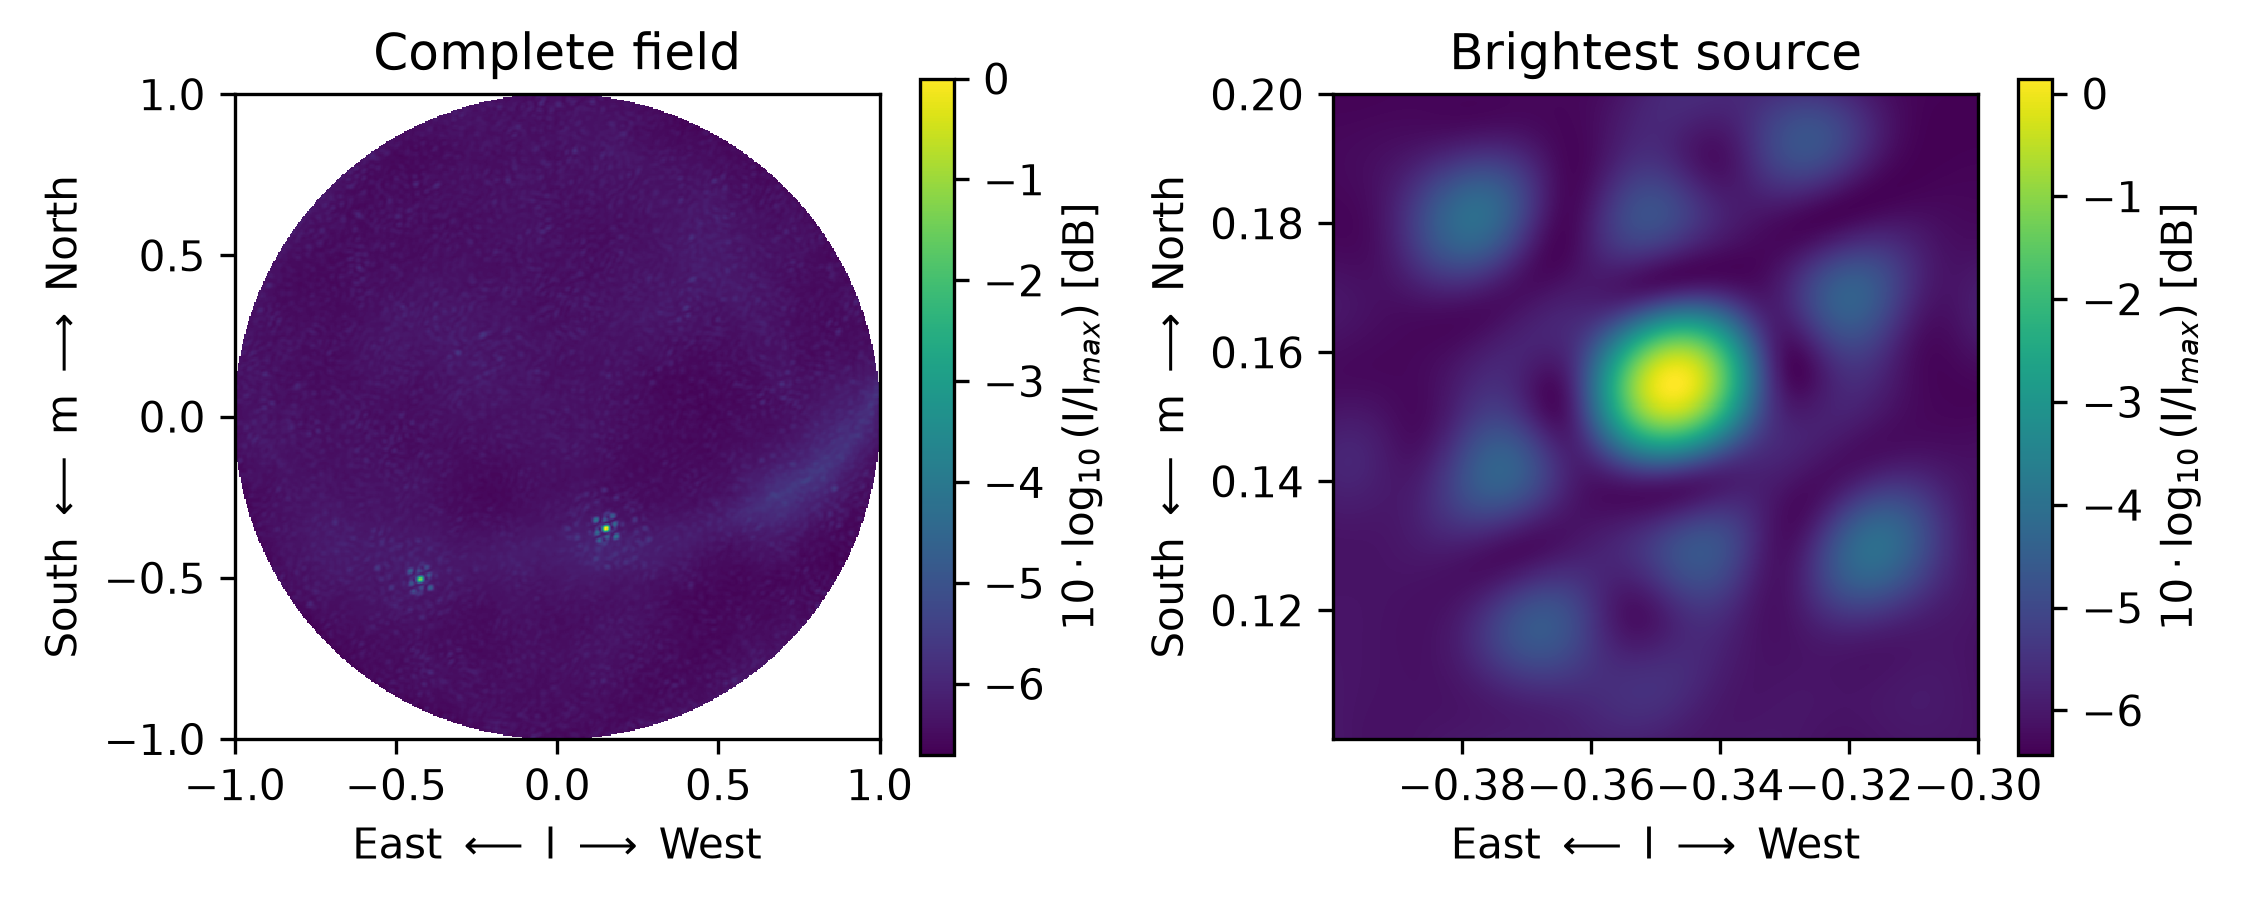
\includegraphics[ width = \textwidth ]{figures/dirty-dual.png}
    \caption{Dirty image obtained with DIRTY algorithm (left) and high-resolution, cropped image near brightest source (right)}
    \label{fig:results-dirty}
\end{figure}
\begin{figure}[!ht]
    \centering
    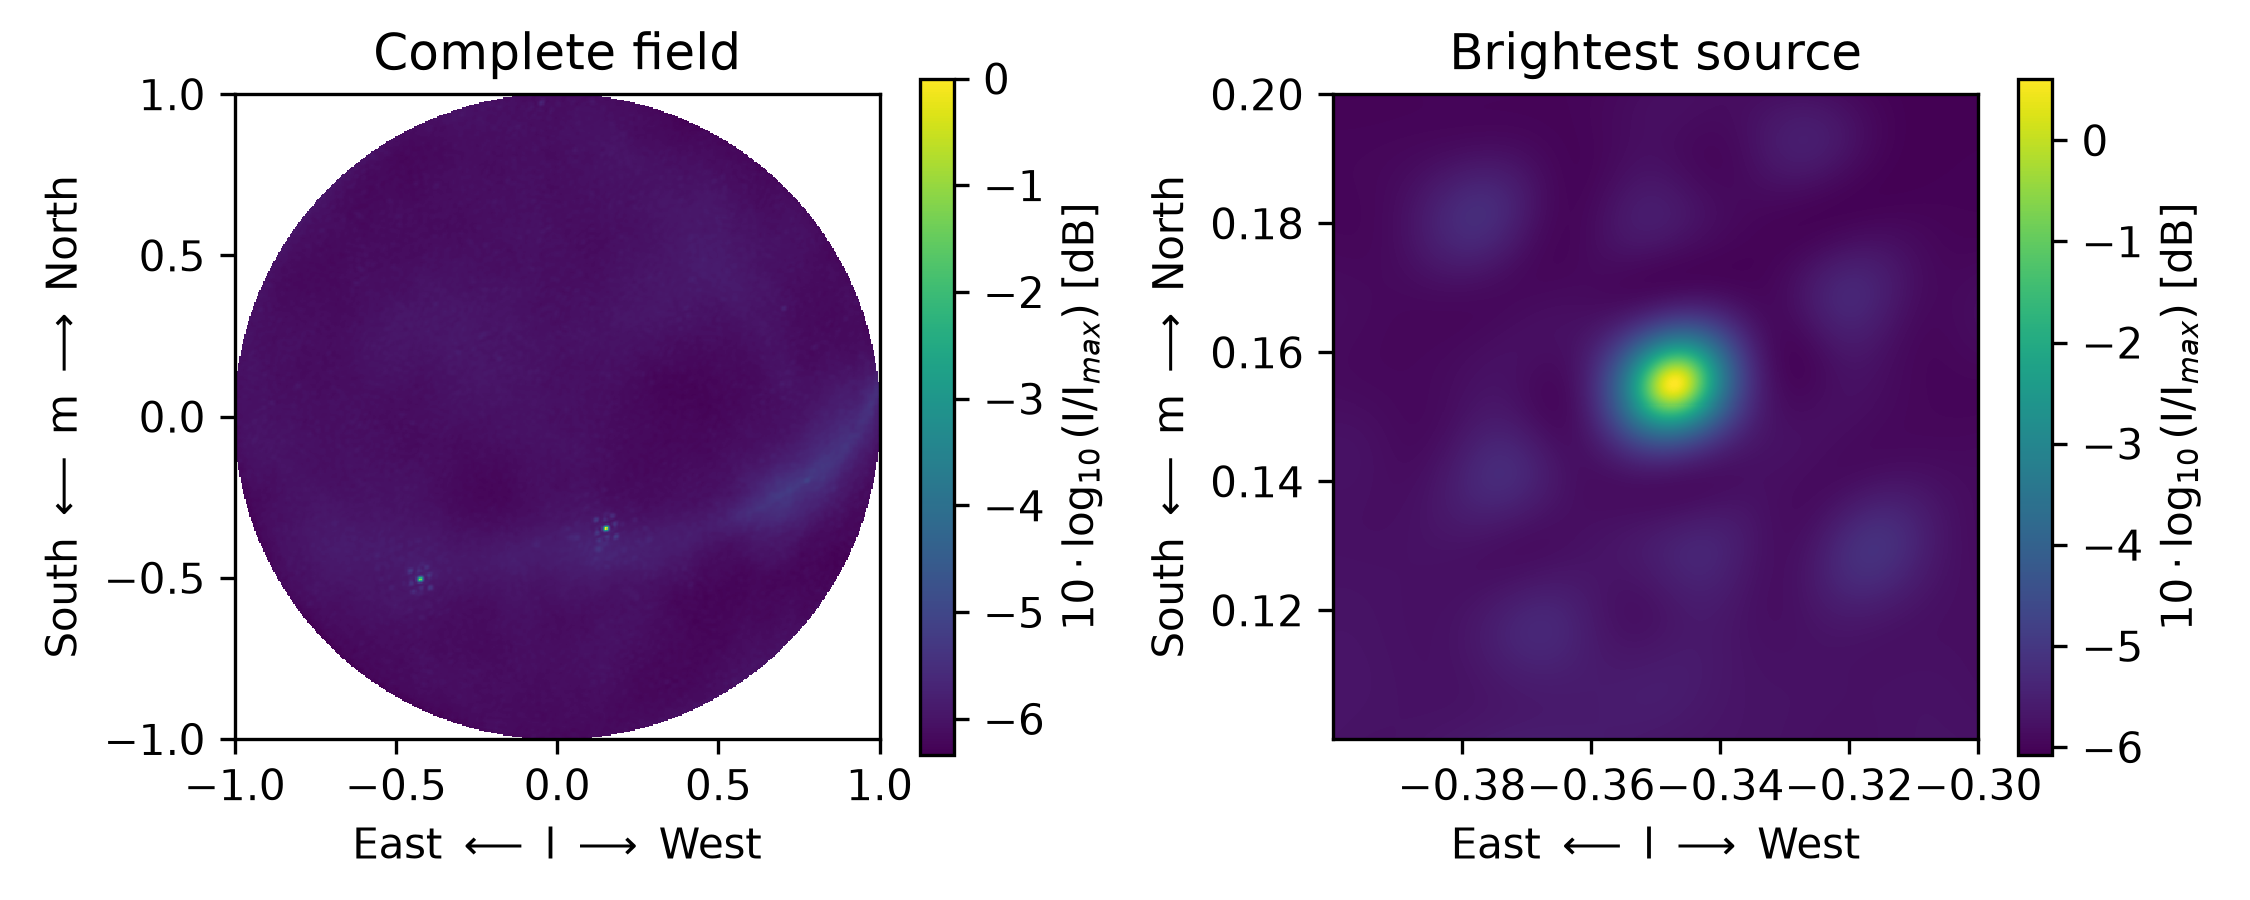
\includegraphics[ width = \textwidth ]{figures/mvdr-dual.png}
    \caption{Dirty image obtained with MVDR algorithm (left) and high-resolution, cropped image near brightest source (right)}
    \label{fig:results-mvdr}
\end{figure}
\begin{figure}[!ht]
    \centering
    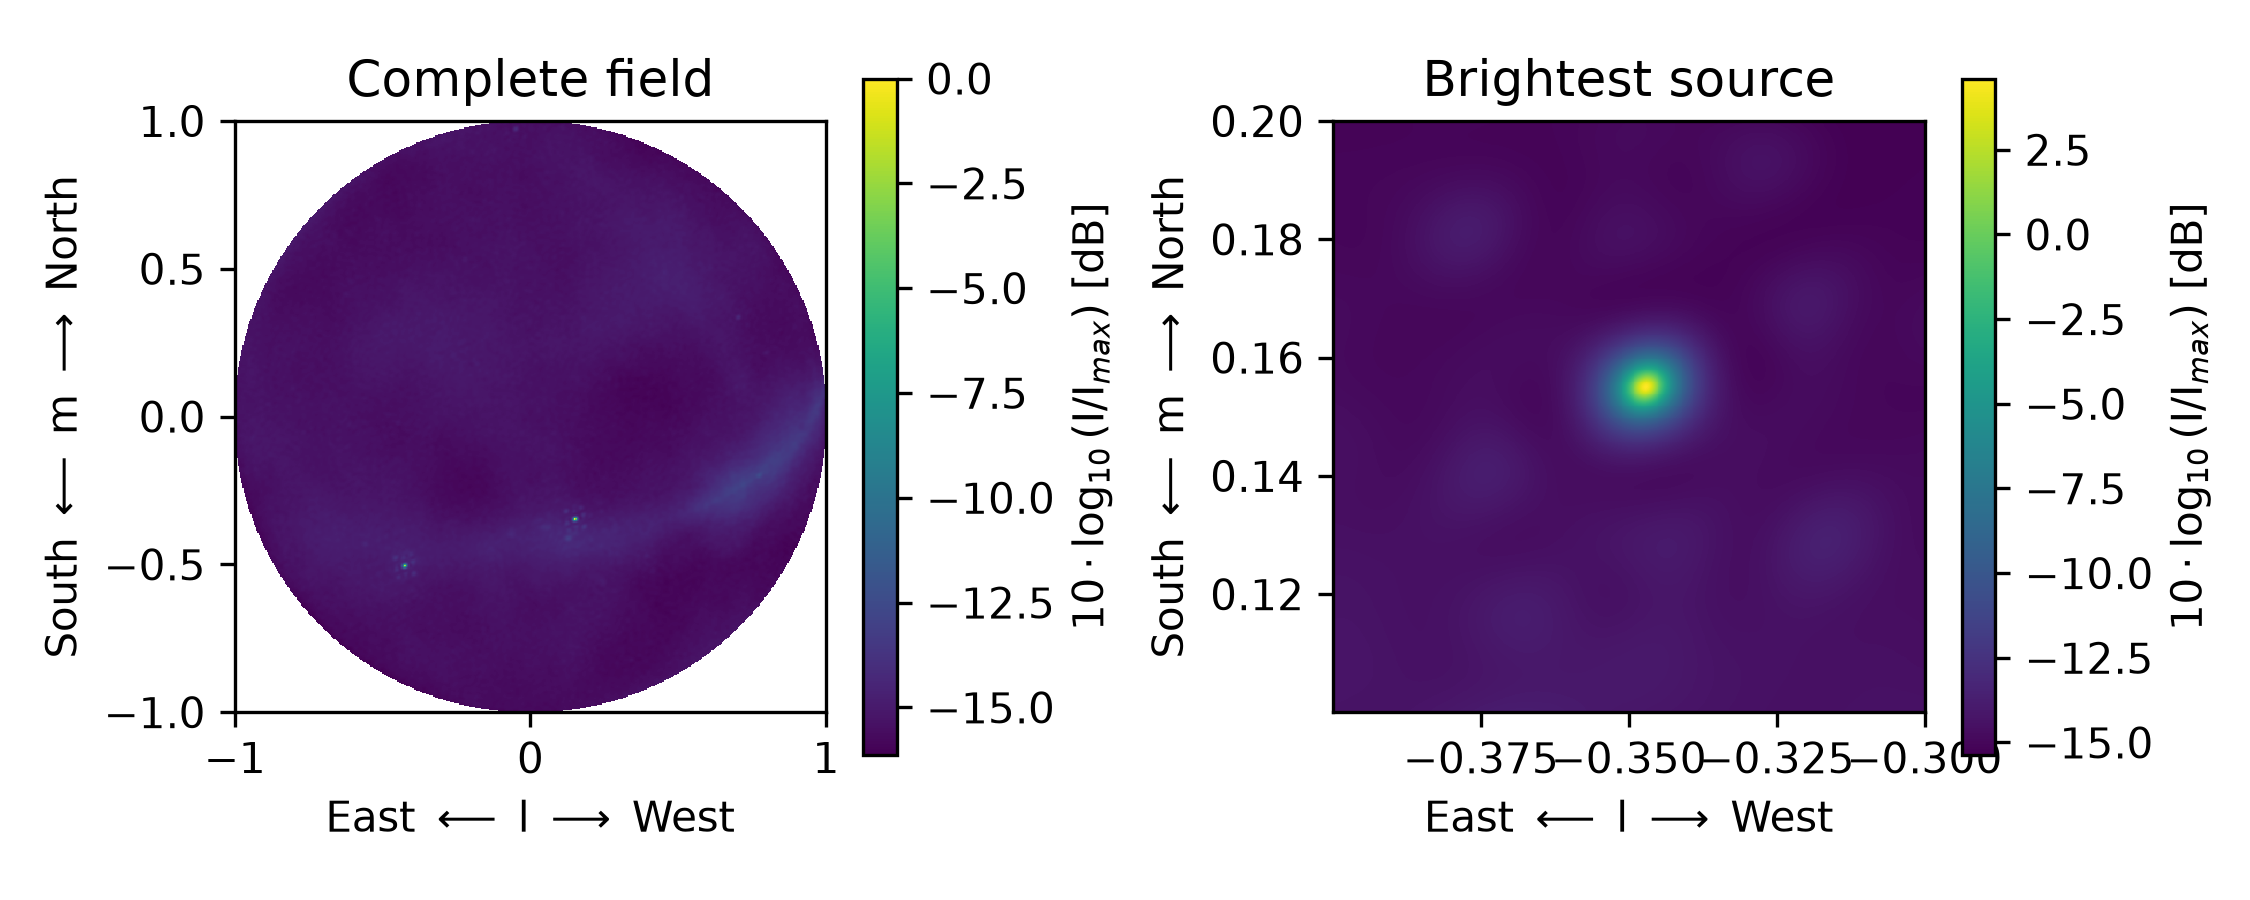
\includegraphics[ width = \textwidth ]{figures/aar-dual.png}
    \caption{Dirty image obtained with AAR algorithm (left) and high-resolution, cropped image near brightest source (right)}
    \label{fig:results-aar}
\end{figure}

A visual inspection of the three images indicates that all the methods manage to resolve the two point sources without issues, as well as what we interpret to be the milky way.
However, a closer inspection reveals that the image produced with DIRTY has clearly stronger sidelobes around the point sources, as well as visible artifacts in the empty regions of the sky.
Quantitatively (see table~\ref{tab:results:metrics}), the $I_{side}/I_{max}$ ratio of DIRTY is around 1.5 higher than MVDR's, and 25 times stronger than AAR's.
This type of behavior is expected from the formulation of the MVDR and AAR algorithms, as their weighing schemes are optimized to minimize contributions from signals not arriving from the direction of observation, which are responsible for sidelobes and background artifacts.

In terms of SNR, although the color scales of figures~\ref{fig:results-dirty} and~\ref{fig:results-mvdr} cover very similar ranges, the results in table~\ref{tab:results:metrics} indicate that the dynamic range of the MVDR image is around 1.6 times larger than DIRTY's.
Such an improvement can be explained by the lack of visible artifacts in the empty regions of the MVDR image, expected from its lower sensitivity to signals not coming from the selected pointing direction.
The improvement in terms of SNR is much more drastic in the AAR image, with 2.74 times the dynamic range of MVDR's.
Such an improvement is consistent with the fact that AAR has been optimized with respect to MVDR to have direction independent background noise, and that the denominator of our expression for the SNR is the standard deviation of a collection of intensities from a large empty region in the image.

\begin{table}[!ht]
    \centering
    \caption{Performance of tested algorithms in terms of their estimated SNR and the FWHM of the brightest source. See section~\ref{s:methods} for information about how these quantities were computed.}
    \begin{tabular}{lccc}
        & SNR [-] & FWHM [-] & $I_{side}/I_{max}$ [-] \\
        \hline
        \hline
        DIRTY & 248.26 & $2.14\cdot 10^{-2}$ & 0.379 \\
        MVDR & 391.76 & $1.26\cdot 10^{-2}$ & 0.265 \\
        AAR & 1074.54 & $3.49\cdot 10^{-3}$ & 0.0150 \\
        \hline
    \end{tabular}
    \label{tab:results:metrics}
\end{table}

Finally, a visual inspection of the cropped images evidences that the width of the PSF of the brightest source decreases from DIRTY to MVDR, and from MVDR to AAR.
The results in table~\ref{tab:results:metrics} support this conclusion, as the FWHM of MVDR is 40\% smaller than that of the MVDR image, and AAR further reduces MVDR's FWHM by a factor of 65\%.

\section{Conclusion}

The purpose of this project was investigating different approaches to generate a dirty image starting from a matrix of complex visibilities derived from LOFAR observations.
Starting from a general beamforming formulation, we implemented three different algorithms: DIRTY, which we took as reference; MVDR, optimized for sidelobe and background noise suppression; and AAR, further optimized with respect to MVDR for direction-independent background noise.
Both a visual inspection of the images and a comparison based on quantitative metrics indicate that the progressive optimizations between algorithms translate into measurable improvements in performance, which become especially obvious for AAR.
While repeating this type of study for other images would be required to ensure that the conclusions generalize, the results of our study suggest that the weighing scheme of AAR offers considerable advantages with respect to the more standard MVDR algorithm, which still performs considerably better than the simple DIRTY algorithm.

\cleardoublepage
\printbibliography

\end{document}
